\documentclass[utf8, russian, hpadding=5mm, vpadding=15mm, floatsection, columnxxvi, columnxxxi, columnxxxii, equationsection, pointsection, footnoteasterisk]{eskdtext}

%доп. пакеты
\usepackage{amsfonts, amsmath, amssymb}	%Для математических штуковин
\usepackage{wallpaper}					%Для вставки сторонних страниц		

%доп. настройки
\bibliographystyle{ugost2008}					%Стиль списка литературы
\graphicspath{{./images/}{./extra_pdf_pages/}}	%Папки с картинками

%на случай, если команда не определена
\newcommand{\No}{\textnumero}

%для определения форматирования нумерации элементов списка литературы
\makeatletter
\renewcommand{\@biblabel}[1]{#1}
\makeatother

%для штампа	
\ESKDtitle{{\Large Название работы}\\ \small Пояснительная записка}
\ESKDsignature{КСУИ.102.4135.001 ПЗ}
\ESKDgroup{\footnotesize Университет ИТМО\\Кафедра СУиИ\\гр.~P4135}
\ESKDauthor{\resizebox{2.22cm}{\height}{Фамилия И.О.}}
\ESKDchecker{\resizebox{2.22cm}{\height}{Фамилия И.О.}}
\ESKDnormContr{\resizebox{2.22cm}{\height}{Фамилия И.О.}}
\ESKDapprovedBy{\resizebox{2.22cm}{\height}{Фамилия И.О.}}

%оступы от заголовков разделов и подразделов
\ESKDsectSkip{section}{7mm}{7mm}
\ESKDsectSkip{subsection}{5mm}{5mm}
\ESKDsectSkip{subsubsection}{3mm}{3mm}


%тело документа
\begin{document}
%\addtocounter{page}{1} %если в документ будут вставлены иные страницы (ТЗ и проч.)
\ESKDthisStyle{empty}
\mbox{}
\ThisLRCornerWallPaper{1}{title_page_1.pdf}
\newpage
%\ESKDthisStyle{empty}
%\mbox{}
%\ThisLRCornerWallPaper{1}{title_page2.pdf}
%\newpage

\ESKDthisStyle{formII}
\tableofcontents
\newpage
\topmargin = 0 mm
\section*{Введение}
\addcontentsline{toc}{section}{Введение}
В~данном документе будет рассказано о процессе разработки системы управления для манипулятора робота Kuka Youbot~\cite{technomatix_kuka_youbot}, дающей ему возможность для совершения двух действий: занятия позиции, при которой его схват будет принимать заданные положение и ориентацию, а также перемещения схвата по заданной траектории\footnote{Здесь и далее, когда речь будет идти о траектории движении схвата, под последней будет подразумеваться не просто кривая, описываемая при этом схватом в пространстве, но таковая, явно параметризованная временем.}.
В~целом содержание пояснительной записки можно описать примерно так:
\begin{itemize}
\item в~разделе~\ref{part_description_of_robot} будут приведены технические сведения о роботе, необходимые для решения поставленных задач;
\item раздел~\ref{part_math_model_of_robot} расскажет о процессе составления математической модели манипулятора, а именно о решении применительно к нему прямой и обратной задач кинематики и о составлении дифференциальных уравнений, описывающих протекающие в роботе электрические и механические процессы;
\item в~разделе~\ref{part_control_systems} речь пойдет о синтезе соответствующих систем управления, о проверке их работоспособности с помощью моделирования, о результатах аппробации на реальном роботе и проч.
\end{itemize}
\newpage

\section{Примеры внутреннего "убранства"}\label{part_example_of_doc_inside}
\subsection{Оформление доп. объектов}\label{part_pasting_of_extra_objects}
\subsubsection{Вставка рисунков}\label{part_pasting_of_figures}
Пример оформления рисунка~--- см.~ниже по тексту.

\begin{figure}[h]
	\centering
	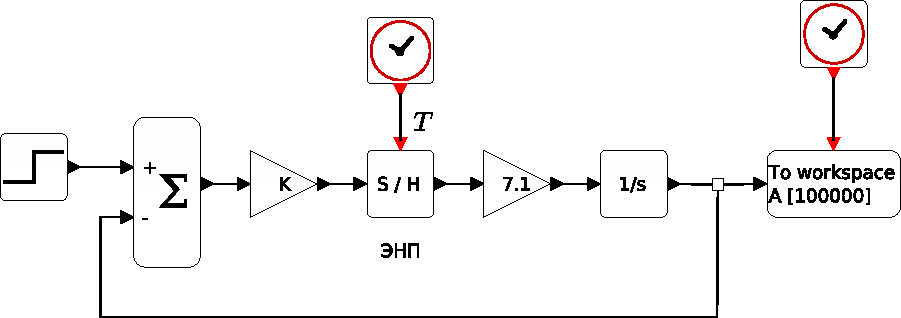
\includegraphics[width=0.7\textwidth]{scheme.pdf}
	\caption{Схема моделирования простенького ОУ.}
	\label{figure_just_example}
\end{figure}


\subsubsection{Вставка таблиц}\label{part_pasting_of_tables}
Пример оформления таблицы~--- см.~ниже по тексту.

\begin{table}[h]
	\caption{Параметры Денавита-Хартенберга.}
	\begin{tabular}{|c|c|c|c|c|}
		\hline
		Звено & $a_i$ & $\alpha_i$ & $d_i$ & $\theta_i$\\
		\hline
		1 & 0 & $\pi/2$ & $l_1$ & $\varphi_1+\pi/2$\\
		\hline
		2  & $l_2$ & $\pi$ & $s_1-2r$ & $\varphi_2-\pi/2$\\
		\hline	
		3 & $l_3$ & $-\pi/2$ & $s_2-2r$ & $-\varphi_3$\\
		\hline
		4 & $l_4$ & $-\pi/2$ & $s_3-2r$ & $-\varphi_4$\\
		\hline
		5 & $l_5$ & $-\pi/2$ & $s_4-2r$ & $-\varphi_5$\\
		\hline
		6 & $l_6$ & $-\pi/2$ & $s_5-2r$ & $-\varphi_6$\\
		\hline
	\end{tabular}
	\label{table_DH_params}
\end{table}


\subsubsection{Вставка формул}\label{part_pasting_of_formulas}
Пример оформления формулы:
\begin{equation}\label{eq_example_of_formula}
	W(s) = \cfrac{T_ms+1}{T_ms^2+T_es+1}
\end{equation}
где $T_m$~--- первая постоянная, а $T_e$~--- вторая.

\subsection{Оформление cсылок}\label{part_editing_of_refs}
Ссылка на раздел~--- \ref{part_example_of_doc_inside}.
Ссылка на подраздел~--- \ref{part_pasting_of_extra_objects}.
Ссылка на что-то меньшее подраздела~--- \ref{part_pasting_of_figures}.
Ссылка на рисунок~--- \ref{figure_just_example}.
Ссылка на таблицу~--- \ref{table_DH_params}.
Ссылка на формулу~--- \eqref{eq_example_of_formula}.
Ссылка на источник~--- \cite{UrcolaIROS08}\footnote{Описание описания источника~--- см.~used\_books.bib.}.
\newpage
\section*{Заключение}
\addcontentsline{toc}{section}{Заключение}
Текст заключения
\newpage
\renewcommand\refname{Список использованных источников}
\providecommand*{\url}[1]{#1} %нужно для описания некоторых источников
\bibliography{used_books}
\ESKDappendix{обязательное}{Название приложения}\label{append_app_example}
Текст приложения
\end{document}